All discussion so far involved either simulated samples, Belle~II data samples with \BtoXsgamma events negligible,
or with the signal region ($\EB\in(1.8,2.7)~\gev$) hidden.
After preparing the analysis on simulation, performing extensive validation and evaluating systematic uncertainties, 
the signal region is ready to be unblinded, as it was shown that no significant biases are expected.
This section presents the results of the analysis.

\subsection{\texorpdfstring{\Mbc}{Mbc} fit results}\label{sec:mbc_fit_results}

Following the \Mbc fitting strategy described in \Cref{sec:fitting_setup} and the model in \Cref{tab:fitting_init_params_updated},
the fits on the signal region of Belle~II data are performed.
They are shown in \Cref{fig:data_fits_signal}.
Together with fits in \Cref{fig:sideband_data_fit}, it gives all the fits for the defined \EB intervals in \Cref{sec:binning}.
The extracted $\mathcal{N}_{\mathrm{CB}}$ are shown in the top right corner of each figure.
\begin{figure}[htbp!]
    \centering
    \subcaptionbox{\label{fig:data_fit_1p8_2p0}}{
        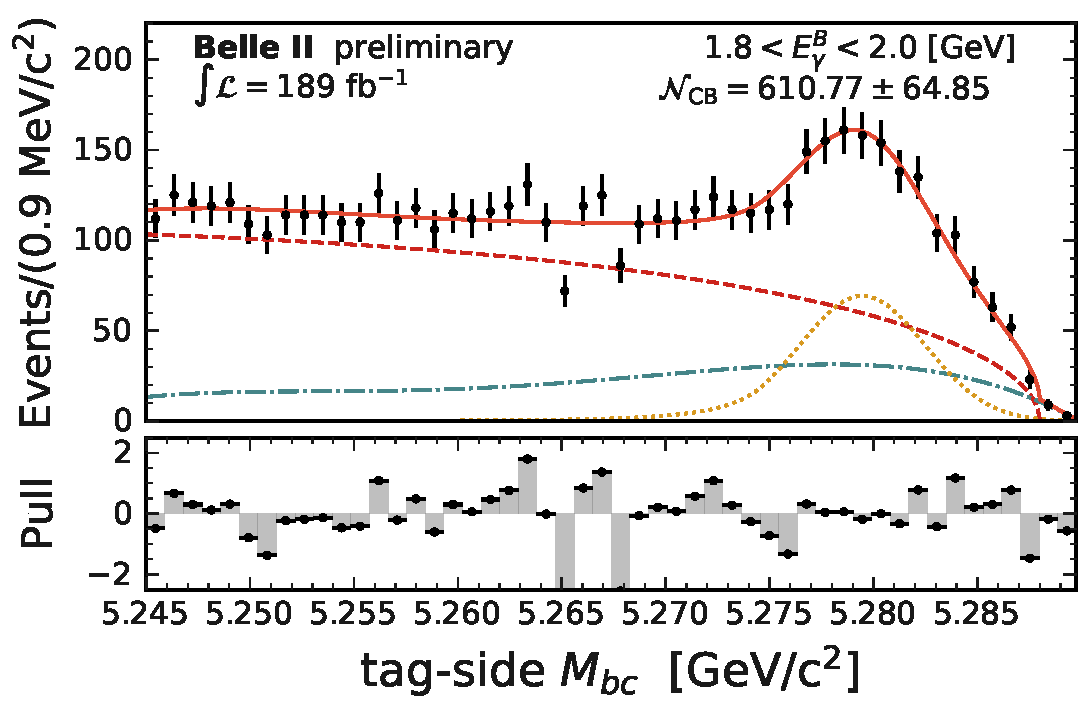
\includegraphics[width=0.3\textwidth]{figures/final_results/data_fits/DATA_MbcFit_1p8to2p0ppdf.pdf}
    }
    \subcaptionbox{\label{fig:data_fit_2p0_2p1}}{
        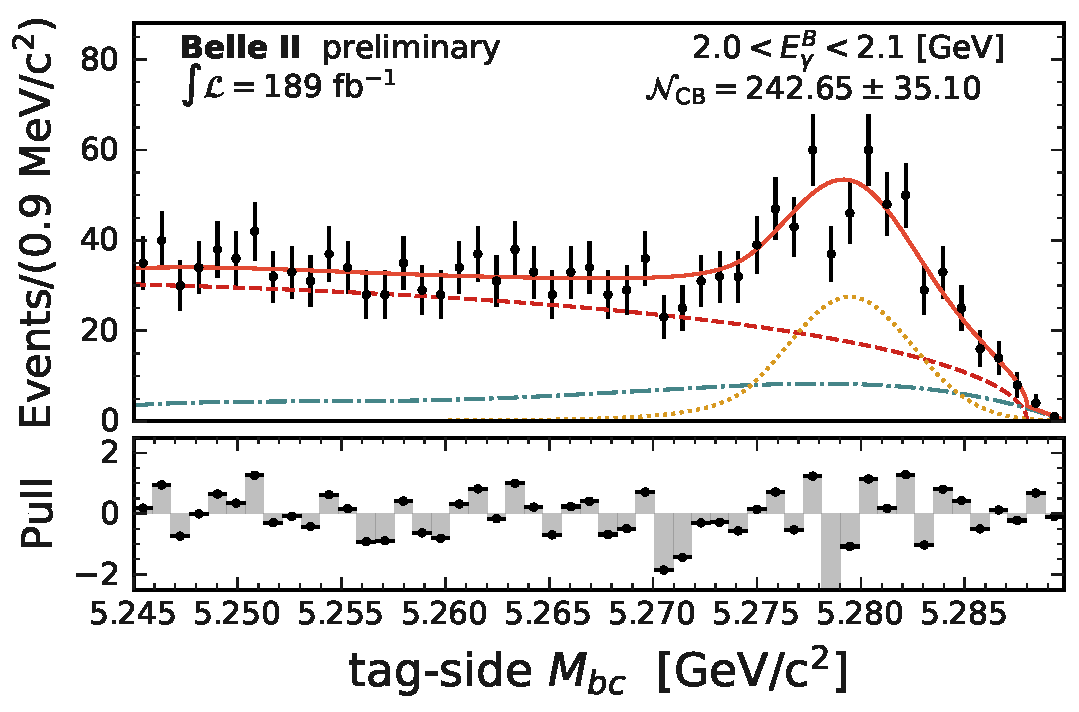
\includegraphics[width=0.3\textwidth]{figures/final_results/data_fits/DATA_MbcFit_2p0to2p1ppdf.pdf}
    }
    \subcaptionbox{\label{fig:data_fit_2p1_2p2}}{
        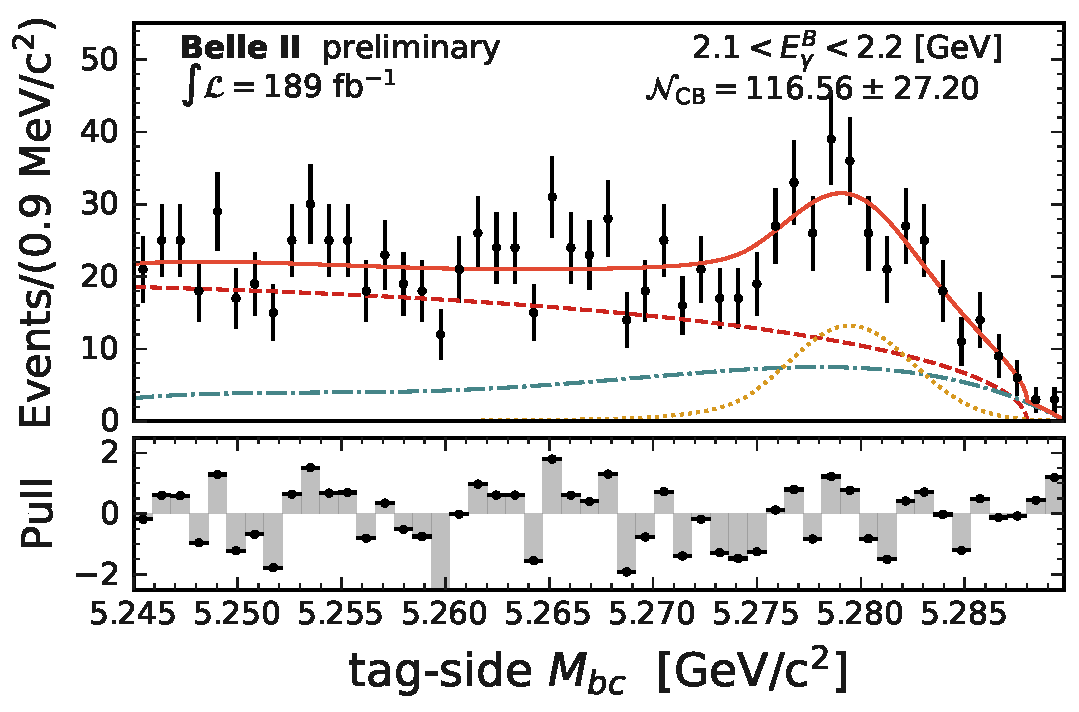
\includegraphics[width=0.3\textwidth]{figures/final_results/data_fits/DATA_MbcFit_2p1to2p2ppdf.pdf}
    }
    \subcaptionbox{\label{fig:data_fit_2p2_2p3}}{
        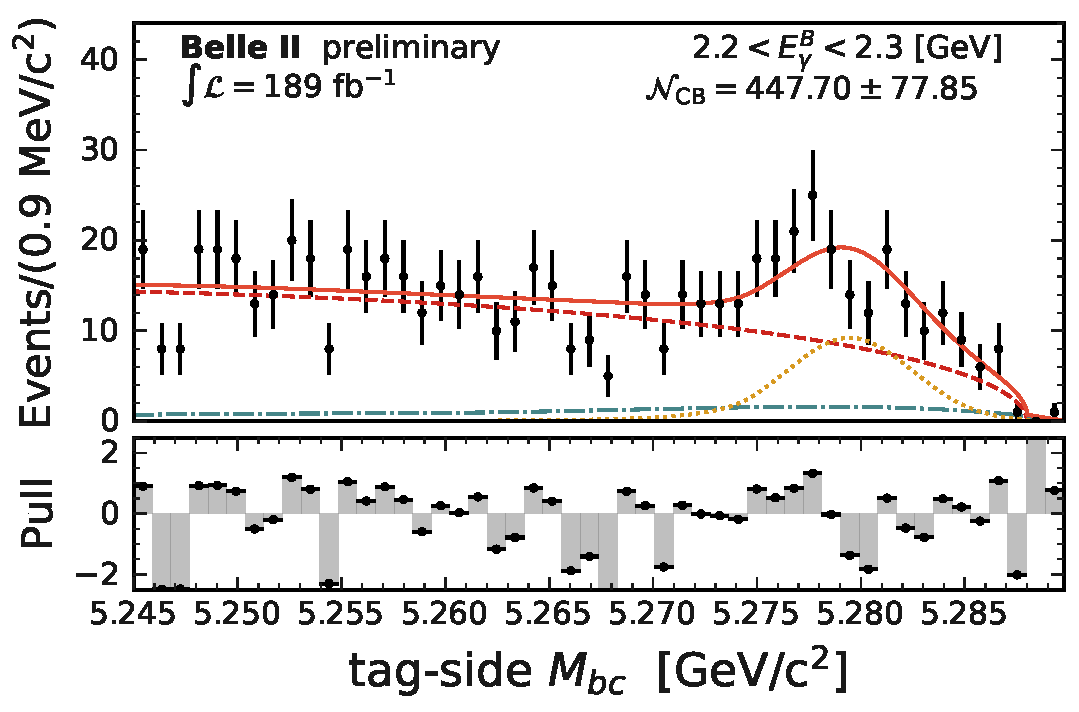
\includegraphics[width=0.3\textwidth]{figures/final_results/data_fits/DATA_MbcFit_2p2to2p3ppdf.pdf}        
    }
    \subcaptionbox{\label{fig:data_fit_2p3_2p4}}{
        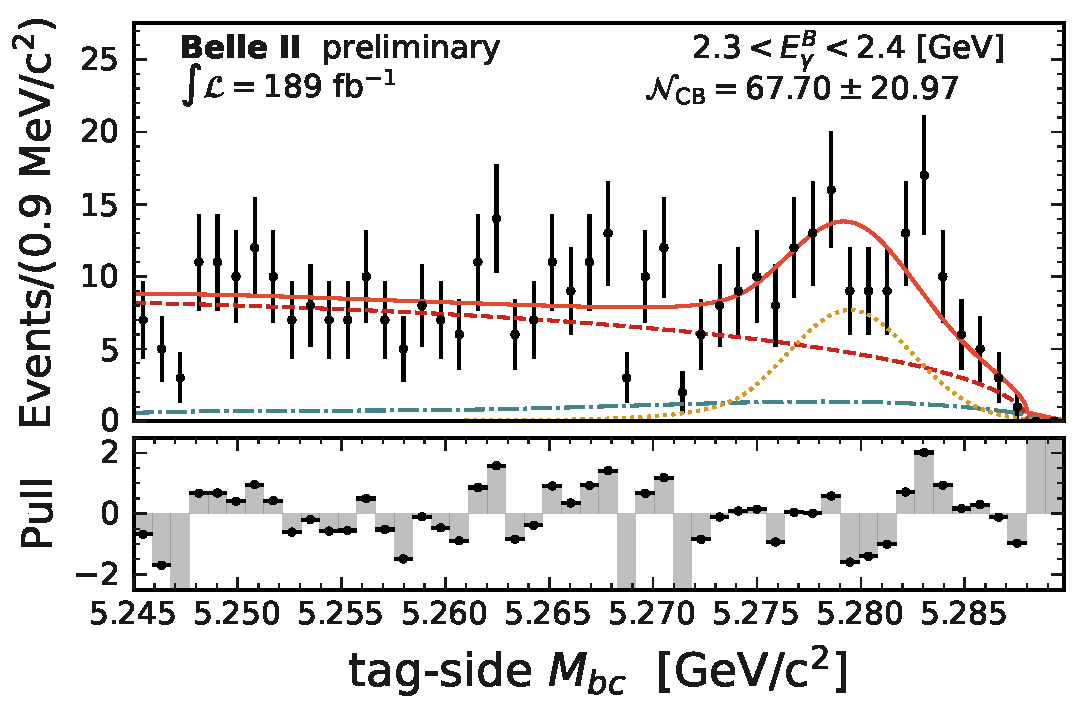
\includegraphics[width=0.3\textwidth]{figures/final_results/data_fits/DATA_MbcFit_2p3to2p4ppdf.pdf}
    }
    \subcaptionbox{\label{fig:data_fit_2p4_2p5}}{
        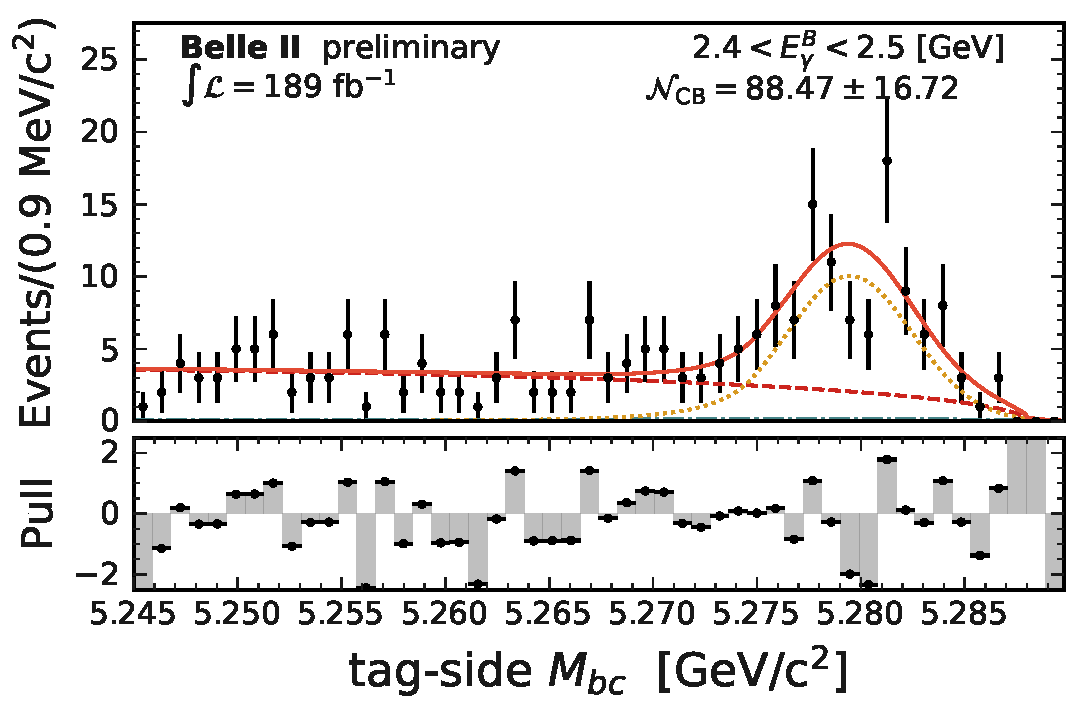
\includegraphics[width=0.3\textwidth]{figures/final_results/data_fits/DATA_MbcFit_2p4to2p5ppdf.pdf}
    }
    \subcaptionbox{\label{fig:data_fit_2p5_2p6}}{
        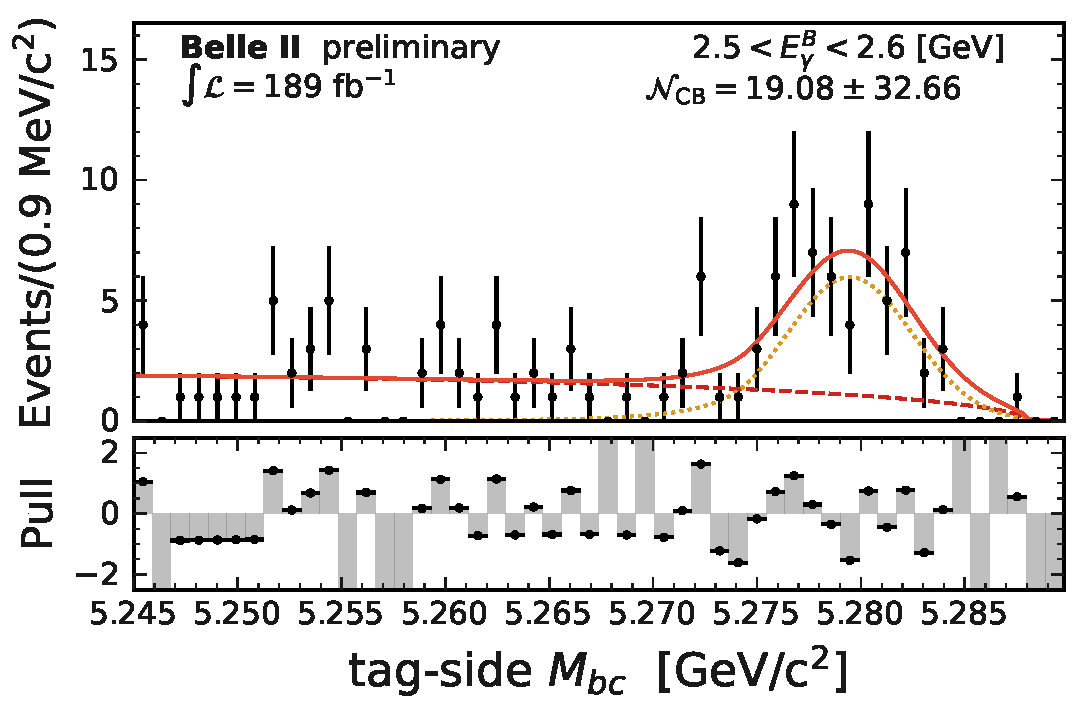
\includegraphics[width=0.3\textwidth]{figures/final_results/data_fits/DATA_MbcFit_2p5to2p6ppdf.pdf}
    }
    \subcaptionbox{\label{fig:data_fit_2p6_2p7}}{
        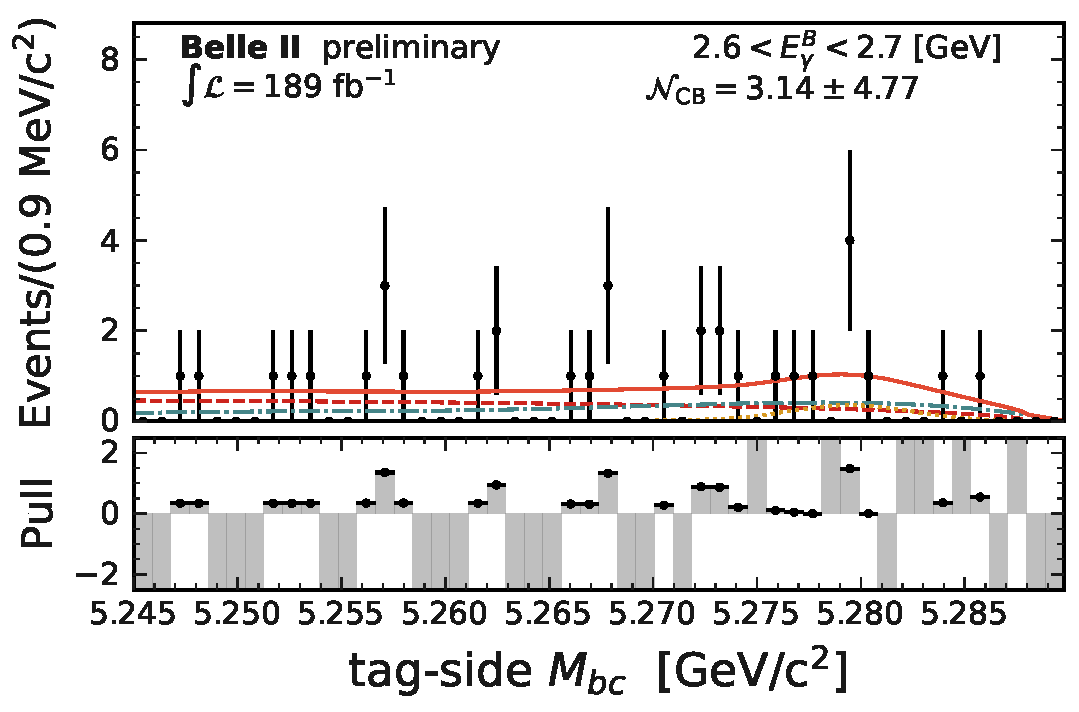
\includegraphics[width=0.3\textwidth]{figures/final_results/data_fits/DATA_MbcFit_2p6to2p7ppdf.pdf}        
    }
    \caption{\label{fig:data_fits_signal}
    The \EB signal region fits on the Belle~II data, based on the fitting model in \Cref{tab:fitting_init_params_updated}.
    The fits are performed as unbinned negative log-likelihood fits.
    The different \EB intervals are shown in the top right corner of each Figure, 
    together with the extracted good tag-\B meson yield, $\mathcal{N}_{\mathrm{CB}}$, which in this case corresponds to remaining good tag-\B backgrounds including \BtoXsgamma and other \BB decay channels.
    The fits outside of the signal region are provided in \Cref{fig:sideband_data_fit}.
    }
\end{figure}

The fit results on Belle~II simulation, with all \BtoXsgamma events removed, are shown in \Cref{fig:nosignal_fits_signal}.
The extracted number of \BB background events is shown in the top right corner of each figure.
These values are corrected, scaled, and are equal to the ones listed in \Cref{tab:background_uncertainties}.
Together with fits in \Cref{fig:sideband_mc_fit}, it gives all the fits for the defined \EB intervals in \Cref{sec:binning}.
\begin{figure}[htbp!]
    \centering
    \subcaptionbox{\label{fig:nosignal_fit_1p8_2p0}}{
        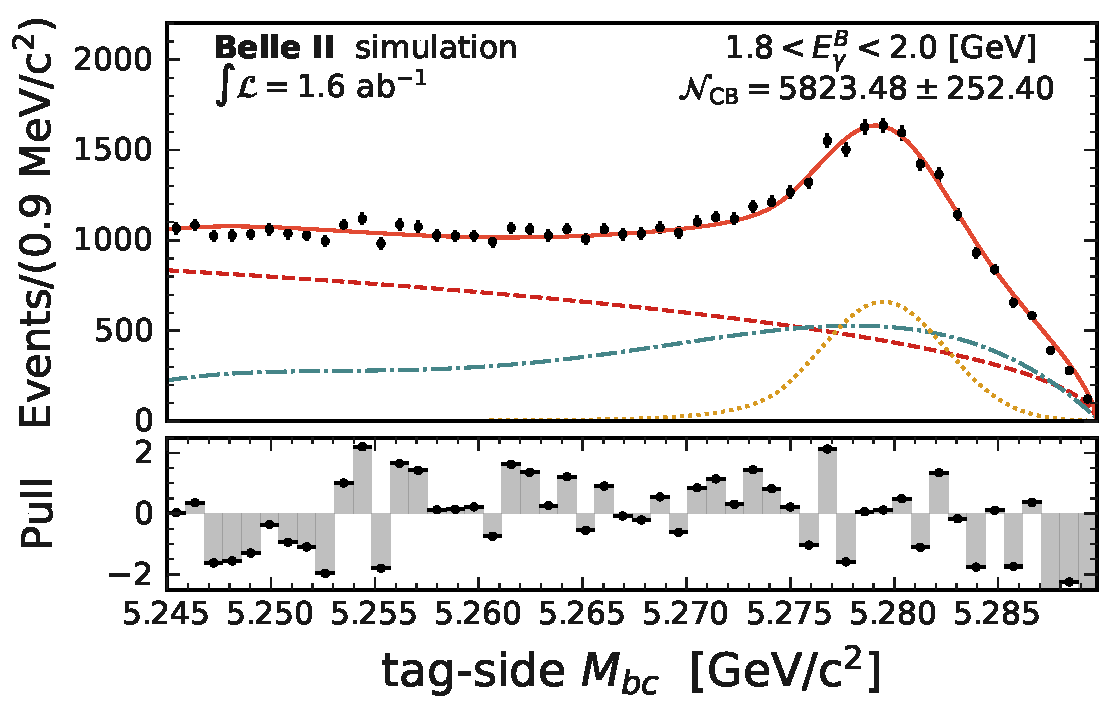
\includegraphics[width=0.3\textwidth]{figures/final_results/mc_fits/NOSIGNALMC_MbcFit_1p8to2p0ppdf.pdf}
    }
    \subcaptionbox{\label{fig:nosignal_fit_2p0_2p1}}{
        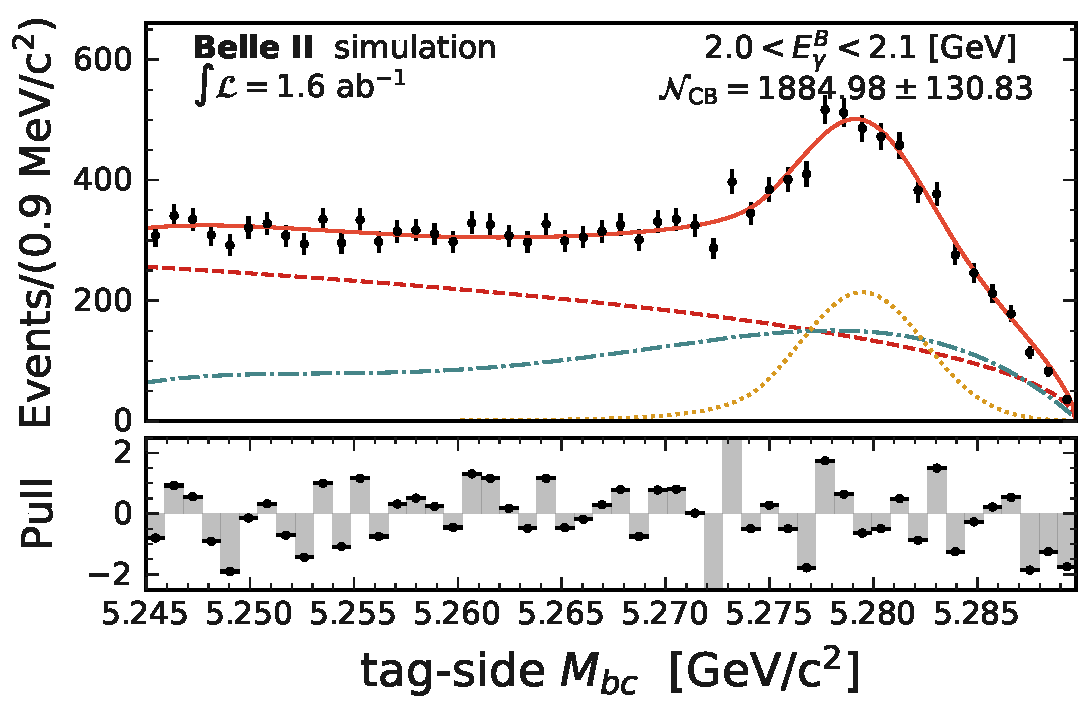
\includegraphics[width=0.3\textwidth]{figures/final_results/mc_fits/NOSIGNALMC_MbcFit_2p0to2p1ppdf.pdf}
    }
    \subcaptionbox{\label{fig:nosignal_fit_2p1_2p2}}{
        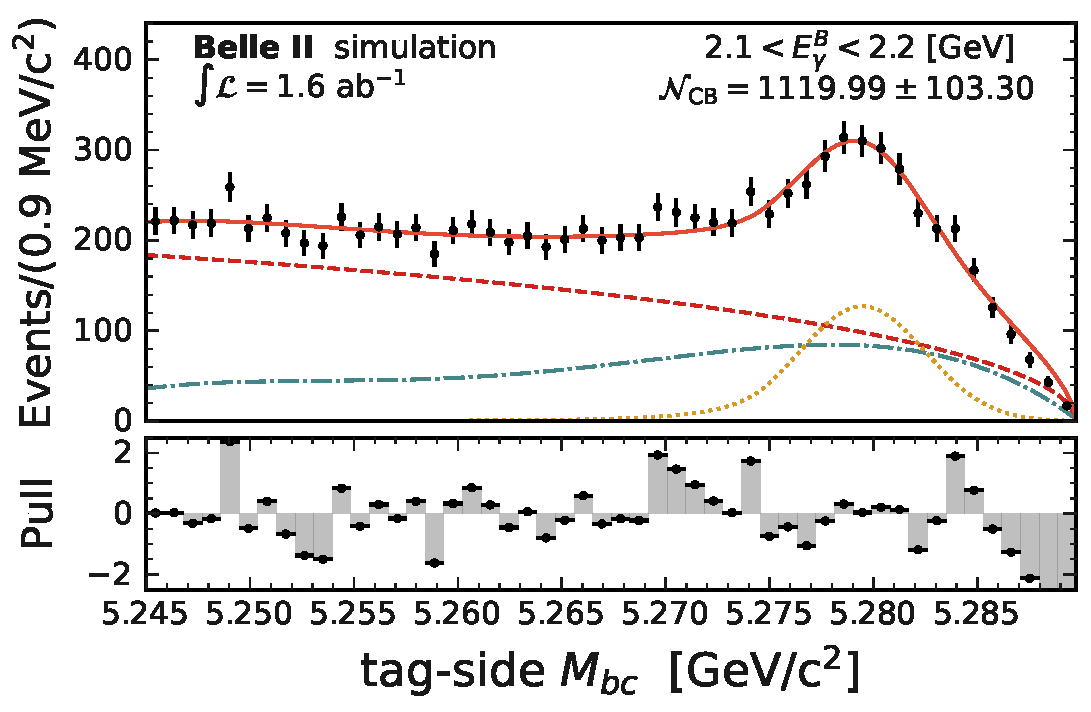
\includegraphics[width=0.3\textwidth]{figures/final_results/mc_fits/NOSIGNALMC_MbcFit_2p1to2p2ppdf.pdf}
    }
    \subcaptionbox{\label{fig:nosignal_fit_2p2_2p3}}{
        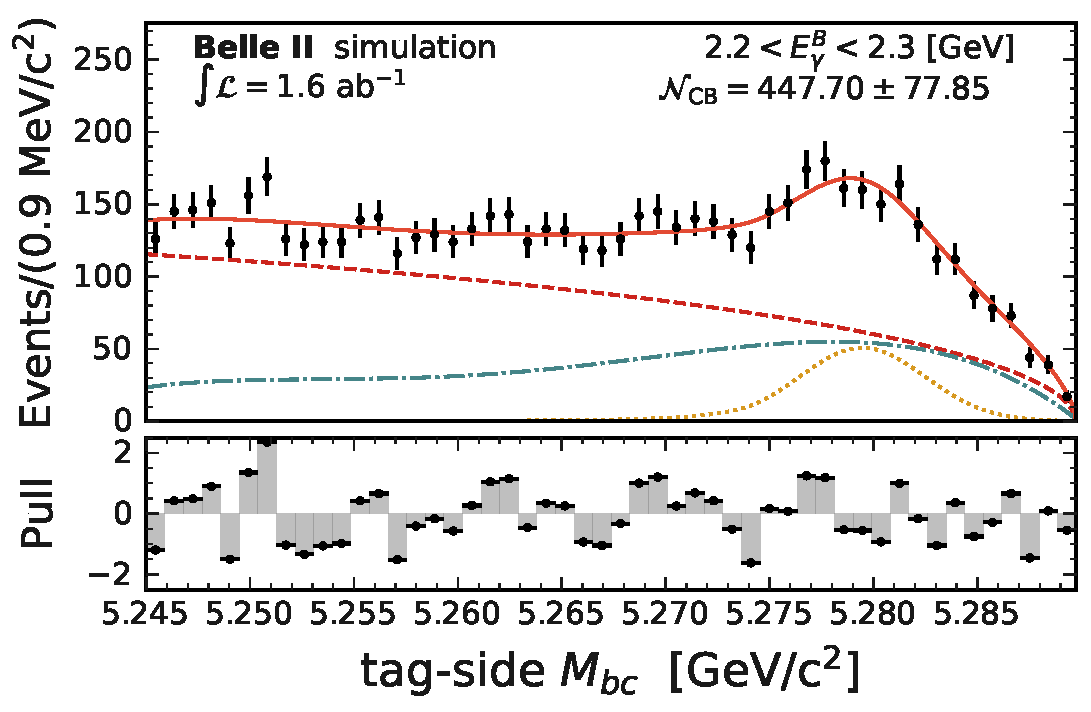
\includegraphics[width=0.3\textwidth]{figures/final_results/mc_fits/NOSIGNALMC_MbcFit_2p2to2p3ppdf.pdf}        
    }
    \subcaptionbox{\label{fig:nosignal_fit_2p3_2p4}}{
        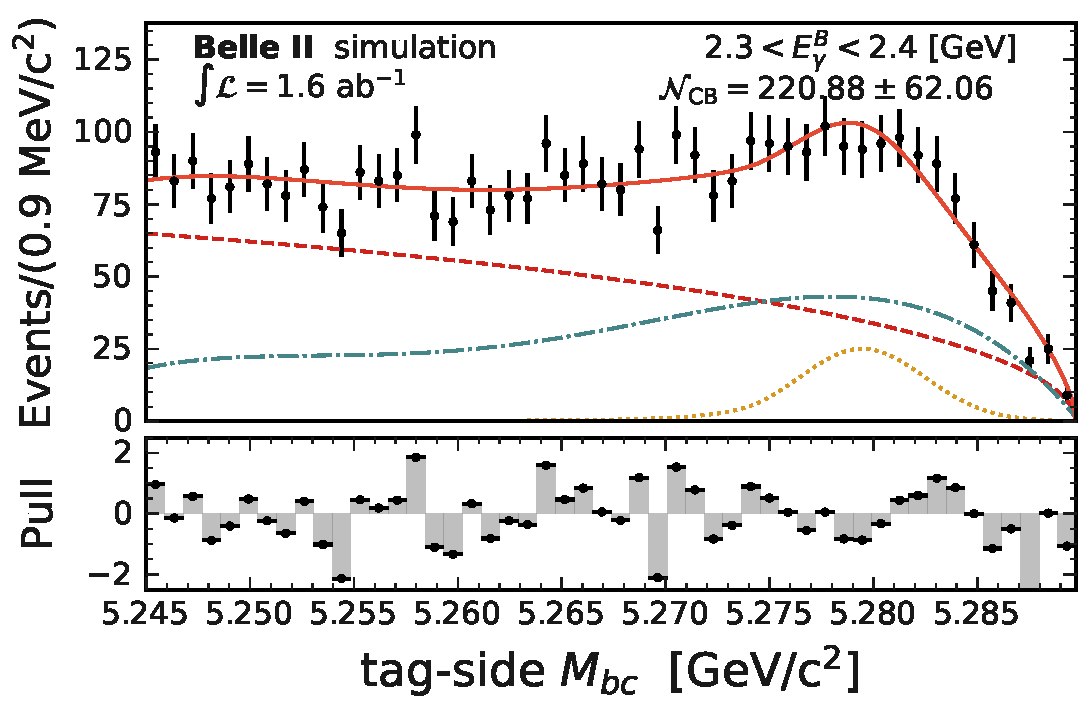
\includegraphics[width=0.3\textwidth]{figures/final_results/mc_fits/NOSIGNALMC_MbcFit_2p3to2p4ppdf.pdf}
    }
    \subcaptionbox{\label{fig:nosignal_fit_2p4_2p5}}{
        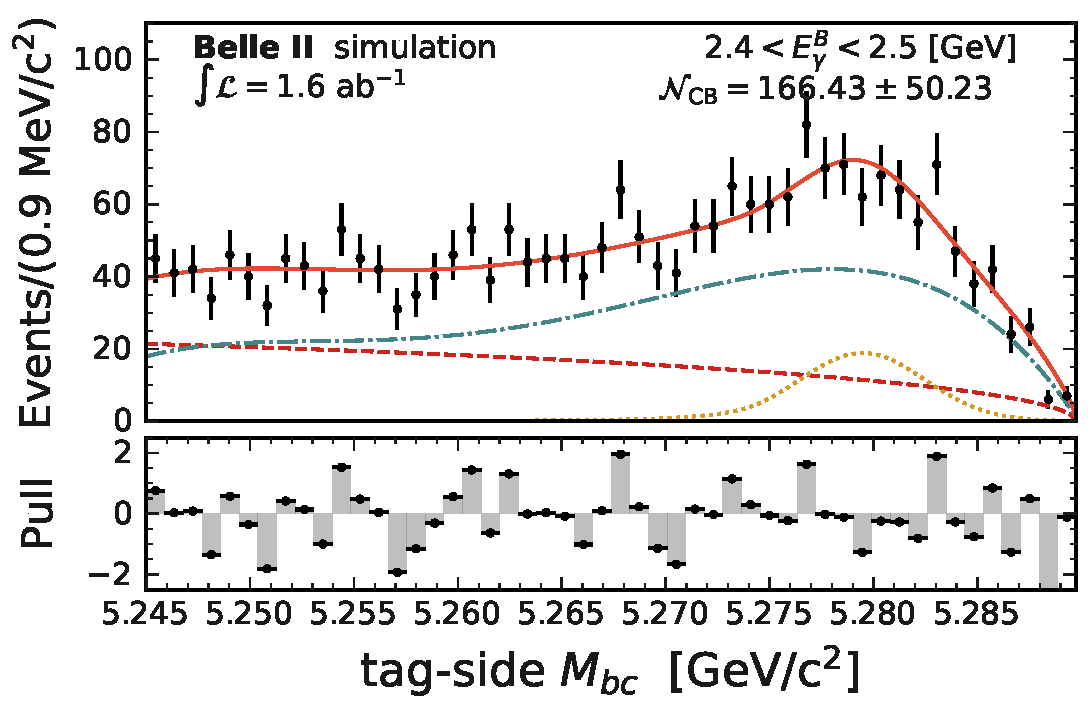
\includegraphics[width=0.3\textwidth]{figures/final_results/mc_fits/NOSIGNALMC_MbcFit_2p4to2p5ppdf.pdf}
    }
    \subcaptionbox{\label{fig:nosignal_fit_2p5_2p6}}{
        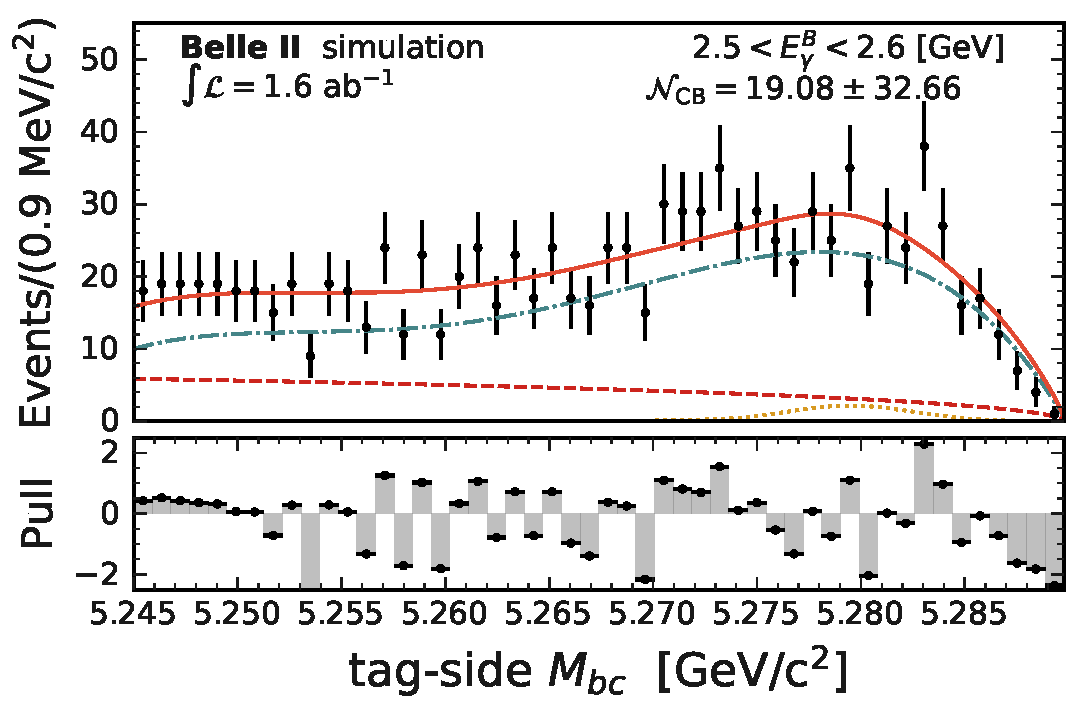
\includegraphics[width=0.3\textwidth]{figures/final_results/mc_fits/NOSIGNALMC_MbcFit_2p5to2p6ppdf.pdf}
    }
    \subcaptionbox{\label{fig:nosignal_fit_2p6_2p7}}{
        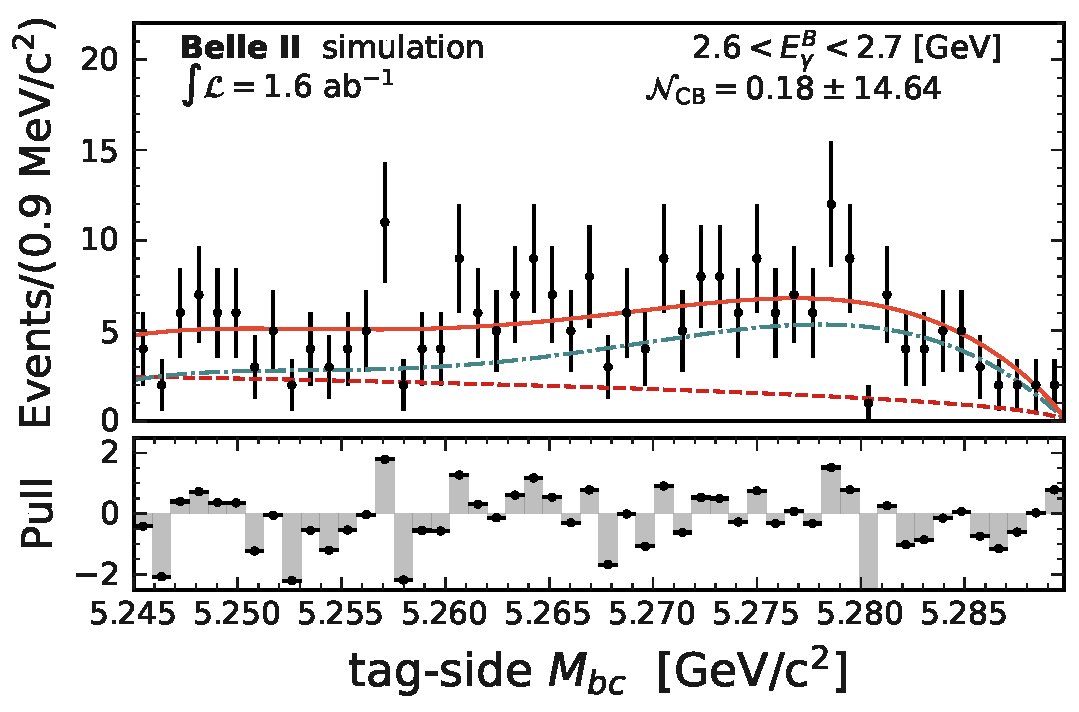
\includegraphics[width=0.3\textwidth]{figures/final_results/mc_fits/NOSIGNALMC_MbcFit_2p6to2p7ppdf.pdf}        
    }
    \caption{\label{fig:nosignal_fits_signal}
    The \EB signal region fits on the Belle~II simulation, where the \BtoXsdgamma events have been removed.
    The fitting model is summarised in \Cref{tab:fitting_init_params_updated}.
    The fits are performed as unbinned negative log-likelihood fits.
    The different \EB intervals are shown in the top right corner of each Figure, 
    together with the extracted good tag-\B meson yield, $\mathcal{N}_{\mathrm{CB}}$, which in this case corresponds only to non-\BtoXsdgamma events with good tag-\B mesons.
    The fits outside of the signal region are provided in \Cref{fig:sideband_data_fit}.
    }
\end{figure}

The number of good tag-\B events, evaluated from fits in Belle~II data (\Cref{fig:sideband_data_fit,fig:data_fits_signal}),
are summarised in \Cref{fig:final_fit_results}.
The figure also includes results from fots on Belle~II simulation with all \BtoXsgamma events removed (\Cref{fig:sideband_mc_fit,fig:nosignal_fits_signal}).
The latter provides the expectations of \BB backgrounds that remain in Belle~II data after the fit.
The simulation is corrected as discussed in \Cref{sec:corrections}, with appropriate uncertainties from \Cref{sec:systematic_uncertainty} included.
The \Cref{fig:final_fit_results_lin} shows the $\mathcal{N}_{\mathrm{CB}}$ in linear axis, which makes the comparison of low-\EB region easier. 
In this region, the number of signal events is expected to be much larger than any contribution from \BtoXsgamma events.
On the other hand, \Cref{fig:final_fit_results_log} shows the results in a logarithmic axis, which makes it evident that an excess over the remaining-\BB background is present.
This excess in data is evidence of \BtoXsdgamma events.

\begin{figure}[htbp!]
    \centering
    \subcaptionbox{\label{fig:final_fit_results_lin}}{
        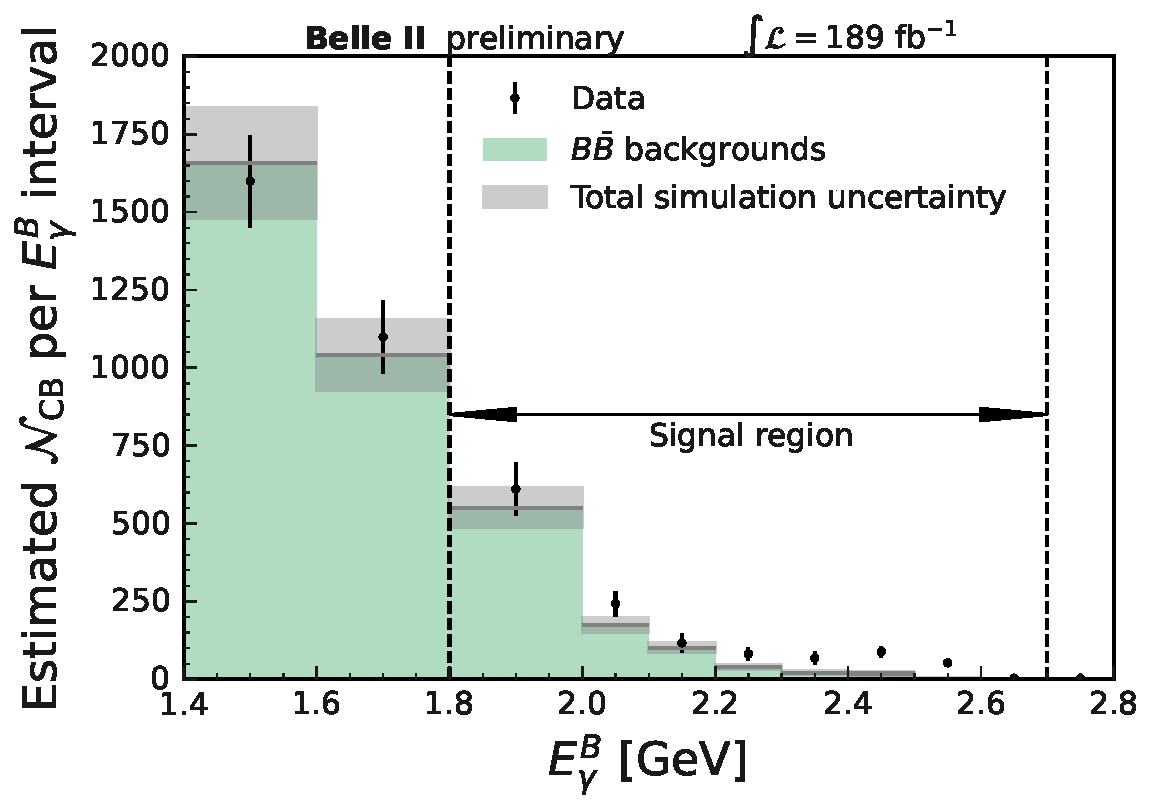
\includegraphics[width=0.45\textwidth]{figures/final_results/background_vs_data_final.pdf}
    }
    \subcaptionbox{\label{fig:final_fit_results_log}}{
        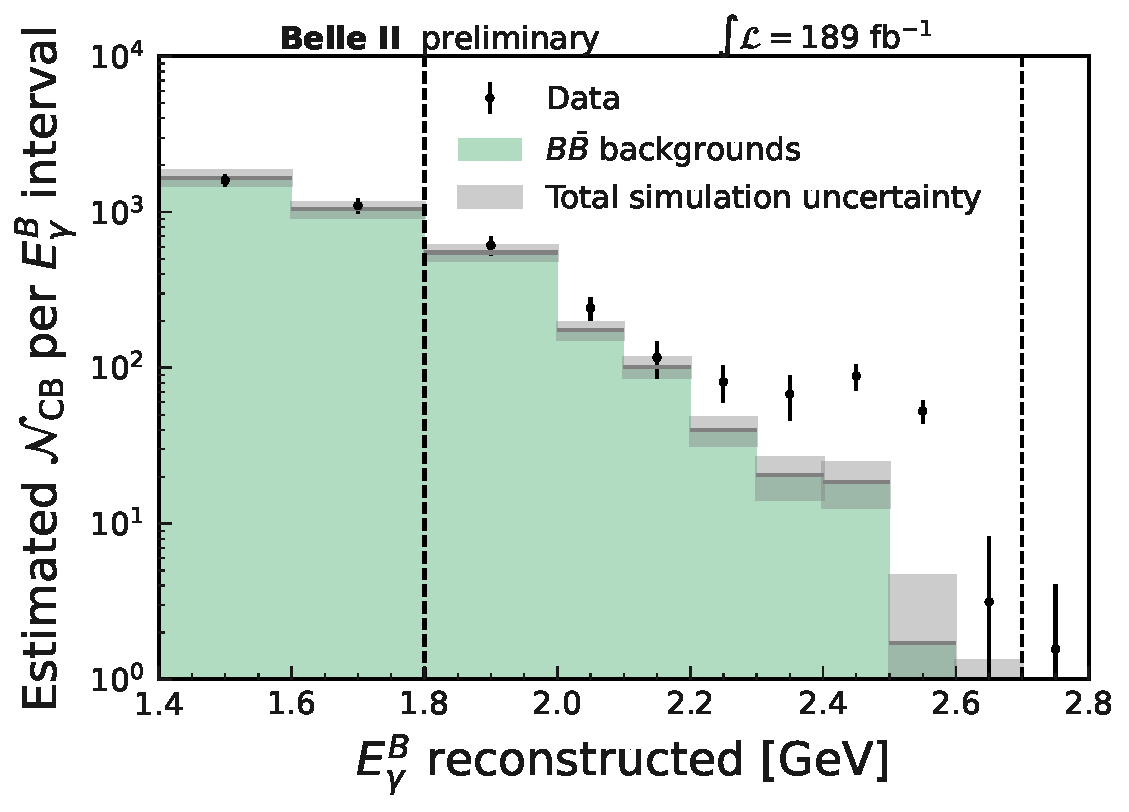
\includegraphics[width=0.45\textwidth]{figures/final_results/background_vs_data_final_log.pdf}
    }
    \caption{\label{fig:final_fit_results}
        The results of fits \Cref{fig:sideband_data_fit,fig:sideband_mc_fit,fig:data_fits_signal,fig:nosignal_fits_signal}.
        All corrections discused in \Cref{tab:correction_table} are applied, 
        and relevant uncertainties from \Cref{tab:background_uncertainties,tab:fit_uncertainties} are included.
        \Cref{fig:final_fit_results_lin} show the results in a linear, whereas \Cref{fig:final_fit_results_log} in a logarithmic axis.
        The excess seen in Belle~II data is evidence of the presence of \BtoXsdgamma events.
    }
\end{figure}

\subsection{Remaining-\texorpdfstring{\BB}{BB} background subtraction results}\label{sec:background_subtraction_results}

The excess that is observed in Belle~II data fits over background-only Belle~II simulation fits is attributed to the presence of \BtoXsdgamma events.
Following the background subtraction strategy shown in \Cref{sec:background_subtraction,sec:background_subtraction_validation_mc},
the remaining good tag-\B meson backgrounds are subtracted.
Simply put, this corresponds to the subtraction of the filled (green) histogram from data points in \Cref{fig:final_fit_results}.
Within uncertainties, the resulting difference can only be accounted by photons that originate in \BtoXsdgamma decays.
The background-subtracted photon energy spectrum is shown in \Cref{fig:subtracted_results}.
\begin{figure}[htbp]
    \subcaptionbox{\label{fig:subtracted_spectrum}}{
        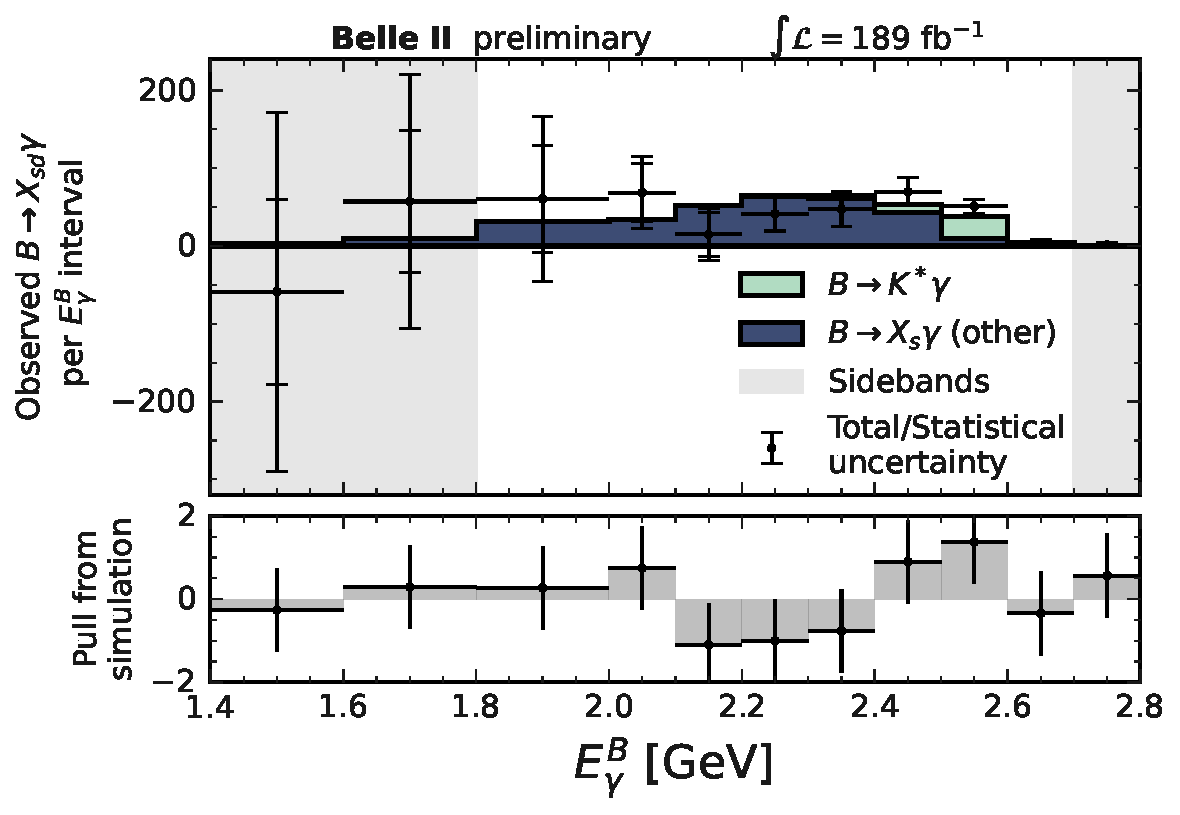
\includegraphics[width=0.45\textwidth]{figures/final_results/reco_spectrum_overlayed.pdf}
    }
    \subcaptionbox{\label{fig:subtracted_spectrum_signal_region}}{
        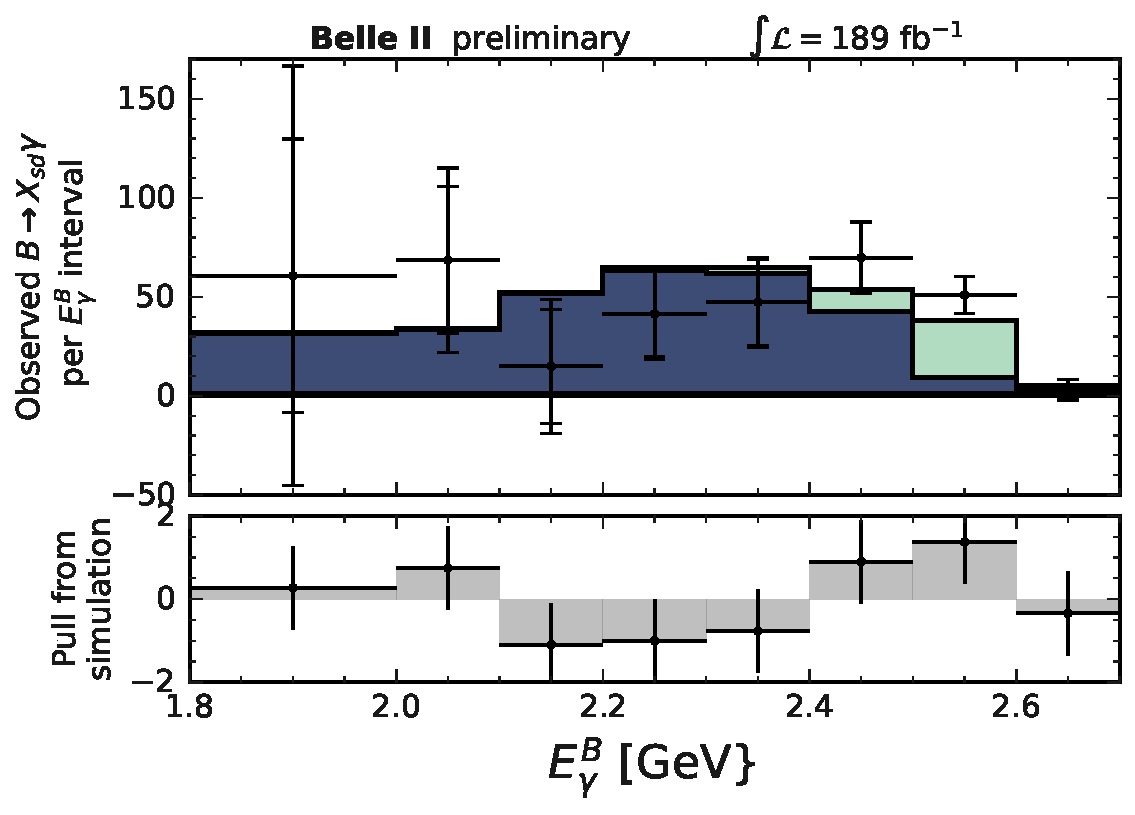
\includegraphics[width=0.45\textwidth]{figures/final_results/reco_spectrum_overlayed_signal_region.pdf}
    }
    \caption{\label{fig:subtracted_results}
        The subtracted spectrum extracted from the Belle~II data after subtracting the remaining non-\BtoXsdgamma background,
        based on results summarised in \Cref{fig:final_fit_results}.
        The total uncertainty, that includes background subtraction and fitting uncertainties is included, without efficiency corrections or unfolding.
        The data points are overlaid the simulated expectation, which shows the hybrid signal-model, defined in \Cref{sec:signal_model}.
        \Cref{fig:subtracted_spectrum} shows all data points, including the sideband region.
        \Cref{fig:subtracted_spectrum_signal_region} is focused only on the signal region.
        The legend is shared for both figures.
    }
\end{figure}

The background subtracted photon energy spectrum include all sysematic uncertainties related 
to background subtraction (\Cref{sec:background_uncertainties})
and fitting uncertainties (\Cref{sec:fit_uncertainties}).
The results agree very well with the simulated expectation from the hybrid signal-model.
The pulls (see \Cref{eq:pull_distribution}) calculated with respect to the hybrid signal-model expectation are evaluated 
and show that all the measured data points agree with the expectation within $1$ to $2\sigma$.

The measured number of events for the signal region in each \EB interval, as well as a cumulative count are given in \Cref{tab:observed_events}.
The statistical as well as a total uncertainty are denoted separately.
The cumulative count is performed starting at the high-\EB intervals and cumulatively adding the contributions from lower-\EB intervals (with systematic uncertainties summed appropriately to their correlation).
This is done as the low-end of the \EB spectrum has the highest uncertainties and the smallest precision.
Using \Cref{eq:btodgamma_subtraction}, the \BtoXsdgamma counts are transformed to \BtoXsgamma event counts.
The cumulative and binned results show excellent agreement with the expectation from the hybrid signal-model.

\begin{table}
    \caption{\label{tab:observed_events}
    The observed number of events (without unfolding) that are consistent with \BtoXsdgamma events in 189~\invfb of Belle~II data.
    The first half of the table shows central value, statistical uncertainty and total uncertainty (in brackets) for each \EB interval.
    The second half of the table shows the cumulative observed number of events (the summation is done from high-\EB, where uncertainties are lower).
    The transformation between \BtoXsdgamma and \BtoXsgamma is performed using the relation in \Cref{eq:btodgamma_subtraction}.
    The expected number of \BtoXsgamma events is provided based on the central values of the hybrid signal-model.
    All results are consistent with the expectations.
    }
    \resizebox{1\textwidth}{!}{
\begin{tabular}{|c||ccc||ccc|}
      \hline
      \multirow{2}{*}{\EB interval [GeV]} & \multicolumn{6}{c|}{Central value $\pm$ Statistical (Total) uncertainty} \\
      \cline{2-7}
       &
      \makecell{Observed\\\BtoXsdgamma events} &
      \makecell{Observed \\\BtoXsgamma events} &
      \makecell{Expected \\\BtoXsgamma value} &
      \makecell{Cumulative\\\BtoXsdgamma events} &
      \makecell{Cumulative\\\BtoXsgamma events} &
      \makecell{Expected \\\BtoXsgamma value} \\
      \hline
        $1.4-1.6$ &  $ -59 \pm 119~(231) $ & $ -56 \pm 114~(221) $& 3 & $ 357 \pm 176~(310) $ & $ 342 \pm 168~(297) $ & 357\\
        $1.6-1.8$ &$ 57 \pm 91~(163) $ & $ 55 \pm 87~(157) $& 10 & $ 416 \pm 129~(207) $ & $ 398 \pm 124~(199) $ & 354 \\
        \hline
        $1.8-2.0$ & $ 61 \pm 69~(106) $ & $ 58 \pm 66~(102) $ & 32 & $ 358 \pm 91~(127) $ & $ 343 \pm 88~(122) $ & 344\\
        $2.0-2.1$ & $ 69 \pm 37~(46) $ & $ 66 \pm 36~(45) $ & 34 & $ 298 \pm 60~(69) $ & $ 285 \pm 57~(68) $ & 312 \\
        $2.1-2.2$ & $ 15 \pm 29~(34) $ & $ 14 \pm 28~(33) $ & 52 & $ 229 \pm 47~(52) $ & $ 220 \pm 45~(50) $ & 278\\
        $2.2-2.3$ & $ 41 \pm 22~(23) $ & $ 40 \pm 21~(22) $ & 65 & $ 214 \pm 37~(39) $ & $ 205 \pm 35~(38) $ & 226\\
        $2.3-2.4$ & $ 47 \pm 22~(23) $ & $ 45 \pm 21~(22) $ & 65 & $ 173 \pm 30~(31) $ & $ 166 \pm 29~(31) $ & 162\\
        $2.4-2.5$ & $ 70 \pm 18~(18) $ & $ 67 \pm 17~(18) $ & 54 & $ 126 \pm 21~(21) $ & $ 120 \pm 20~(21) $ & 97\\
        $2.5-2.6$ & $ 51 \pm 9~(9) $ & $ 49 \pm 9~(9) $     & 38 & $ 56 \pm 11~(11) $ & $ 53 \pm 10~(11) $ & 43\\
        $2.6-2.7$ & $ 3 \pm 5~(5) $ & $ 3 \pm 5~(5) $       & 5& $ 5 \pm 6~(6) $ & $ 4 \pm 5~(6) $ & 5\\
        \hline
        $>2.7$   & $ 2 \pm 2~(2) $ & $ 1 \pm 2~(2) $       & 0 & $ 2 \pm 2~(2) $ & $ 1 \pm 2~(2) $ & 0\\
        \hline
\end{tabular}
}
\end{table}


\subsection{Partial branching fraction measurement results}\label{sec:partial_branching_fraction_results}

The measurement results provided in \Cref{tab:observed_events} and visualised in \Cref{fig:subtracted_spectrum},
are used to calculate the pratial branching fractions of \BtoXsgamma decays.
To this end they are corrected for efficiency and unfolded.
The efficiency used for the calculations is provided in \Cref{sec:signal_selection_uncertainties}, 
whereas the unfolding factors and strategy are described in \Cref{sec:unfolding_systematic}.
Note that up until now \EB and $\tilde{E}_{\gamma}^B$ was used to explicitly differentiate
the measured and the `true' (unfolded) photon-energy, respectively.
\textit{In the following two sections only} the \EB notation is used to denote the unfolded photon-energy (i.e. the tilde notation is omitted).

Combining all the results presented in this thesis leads to the following equation for the partial branching fraction:
\begin{equation}\label{eq:branching_fraction}
    \frac{\Delta\mathcal{B}(\BtoXsgamma)_i}{\Delta {E^B_{\g}}_{,i}} = \frac{\mathcal{U}_i\times\left(\mathcal{N}^{\mathrm{DATA}}_{\mathrm{CB},i} - 
                                                                              \mathcal{N}^{\mathrm{non-}\BtoXsdgamma}_{\mathrm{CB},i} - 
                                                                              N_i^{\BtoXdgamma}\right)}
                                                         {\varepsilon_i \times N_B},
\end{equation}
where (left to right, top to bottom)
\begin{itemize}
    \item $i$ is a given \EB interval,
    \item $\mathcal{U}_i$ is an unfolding factor for interval $i$, based on \Cref{tab:unfolding_uncertainties},
    \item $\mathcal{N}^{\mathrm{DATA}}_{\mathrm{CB},i}$ is the number of good tag-\B mesons in Belle~II data for interval $i$.
    These values are given in XXXX.
    \item $\mathcal{N}^{\mathrm{non-}\BtoXsgamma}_{\mathrm{CB},i}$ is the number of good tag-\B meson candidates where the signal \B meson does not decay as \BtoXsdgamma, evaluated in Belle~II simulation (corrected for differences in luminosity and modelling) for an interval $i$.
    These values are given in \Cref{tab:background_uncertainties}.
    \item $N_i^{\BtoXdgamma}$ is the number of \BtoXdgamma events contributing in for an interval $i$,
    \item $\varepsilon_i$ is the factorised signal efficiency for interval $i$, defined in \Cref{eq:factorisable_signal_efficiency}, 
    with values taken from \Cref{tab:signal_selection_uncertainties} and \Cref{eq:tag_efficiency_with_uncertainty},
    \item $N_B$ as the number of $B$ mesons in the analysed Belle~II data sample, as given in \Cref{eq:b_meson_count}.
\end{itemize}

The results of the calculations based on \Cref{eq:branching_fraction} with all 
results discussed and derived in this thesis are shown in \Cref{tab:partial_branching_fractions}.
The statistical and systematic uncertainty are included, where the latter is broken down to four categories presented in \Cref{sec:systematic_uncertainty}.
The calculations are only performed for the signal region $\EB\in(1.8,2.7)~\gev$ where the unfolding factors are available.
Furthermore, the $\EB\in(2.6,2.7)~\gev$ interval is not given in \Cref{tab:partial_branching_fractions}, 
because the unfolding factor for it is 0 (see \Cref{tab:unfolding_uncertainties}).

\begin{table}[htbp!]
    \centering
    \caption{\label{tab:partial_branching_fractions}
    Results of the partial branching fraction measurement presented in this thesis, based on \Cref{eq:branching_fraction}. 
    The first part of the table shows the partial branching fractions for each \EB interval, their statistical and systematic uncertainty components.
    The second part of the table shows the breakdown of the systematic uncertainty, into groups that are defined in \Cref{sec:systematic_uncertainty}. 
    Statistical uncertainties remain the dominant component in the analysis.
    Note that signal efficiency and background modelling uncertainties are correlated due to the same correction factors used (see \Cref{sec:corrections}).
    }
    \resizebox{1\textwidth}{!}{
    \begin{tabular}{|c|ccc||cccc|}
    \hline
    \multirow{2}{*}[-6pt]{\EB interval [\gev]} &
    \multirow{2}{*}[-6pt]{$\frac{\Delta\mathcal{B}(\BtoXsgamma)_i}{\Delta {E^B_{\g}}_{,i}} (10^{-4})$} &
    \multirow{2}{*}[-6pt]{\makecell{Statistical\\uncertainty} ($10^{-4}$)} &
    \multirow{2}{*}[-6pt]{\makecell{Systematic\\uncertainty} ($10^{-4}$)}& 
    \multicolumn{4}{c|}{Systematic uncertainty group} \\
    \cline{5-8}
    & & & &        
    \makecell{Background \\ modelling} &
    \makecell{\Mbc fit \\ model} & 
    \makecell{\BtoXsgamma \\efficiency} & 
    \makecell{Other\\uncertainties}\\
    \hline
    $1.8-2.0$  &  0.48 & $\pm0.54$ & $\pm0.64$ & 0.49 & 0.42 & 0.03 & 0.09 \\
    $2.0-2.1$  &  0.57 & $\pm0.31$ & $\pm0.25$ & 0.17 & 0.17 & 0.06 & 0.07 \\
    $2.1-2.2$  &  0.13 & $\pm0.26$ & $\pm0.16$ & 0.11 & 0.13 & 0.01 & 0.01 \\
    $2.2-2.3$  &  0.41 & $\pm0.22$ & $\pm0.10$ & 0.04 & 0.07 & 0.05 & 0.02 \\
    $2.3-2.4$  &  0.48 & $\pm0.22$ & $\pm0.10$ & 0.02 & 0.06 & 0.06 & 0.05 \\
    $2.4-2.5$  &  0.75 & $\pm0.19$ & $\pm0.14$ & 0.02 & 0.04 & 0.09 & 0.09 \\
    $2.5-2.6$  &  0.71 & $\pm0.13$ & $\pm0.10$ & 0.00 & 0.02 & 0.09 & 0.04  \\
    \hline
    \end{tabular}
}
\end{table}

Comparing the systematical and statistical uncertainties, the results in \Cref{tab:partial_branching_fractions} 
are largely statistically dominated in all \EB intervals.
Although the statistical uncertainty dominates, the systematic uncertainty comparable to it in high-\EB intervals.
The results shown in the table show that the background modelling is
and fit-modelling uncertainties are dominant in the low-\EB region.
On the other hand, signal selection modelling uncertainties and other uncertainties (particularly the unfolding uncertainty) become dominant at high-\EB.
These observations are consistent with the fact that the signal-to-background ratio grows with decreasing \EB (as seen in e.g. \Cref{tab:expected_events}),
and the fact that the number of \BtoXsgamma events is larger at higher \EB values.

The systematic uncertainties in \Cref{tab:partial_branching_fractions} are correlated:
both between different systematic uncertainty groups (i.e. signal selection efficiencu and background modelling)
and between different \EB bins.
These correlations, as discussed in \Cref{sec:systematic_uncertainty}, are combined and evaluated.
The correlation matrix is shown in \Cref{fig:correlation_uncertainty_matrix}.
The statistical and systematic component is merged here.
As the results have a large statistical uncertainty component, the correlation of uncertainties is found to be low.

\begin{figure}[htbp!]
    \centering
    \subcaptionbox{\label{fig:partial_branching_fraction}}{
        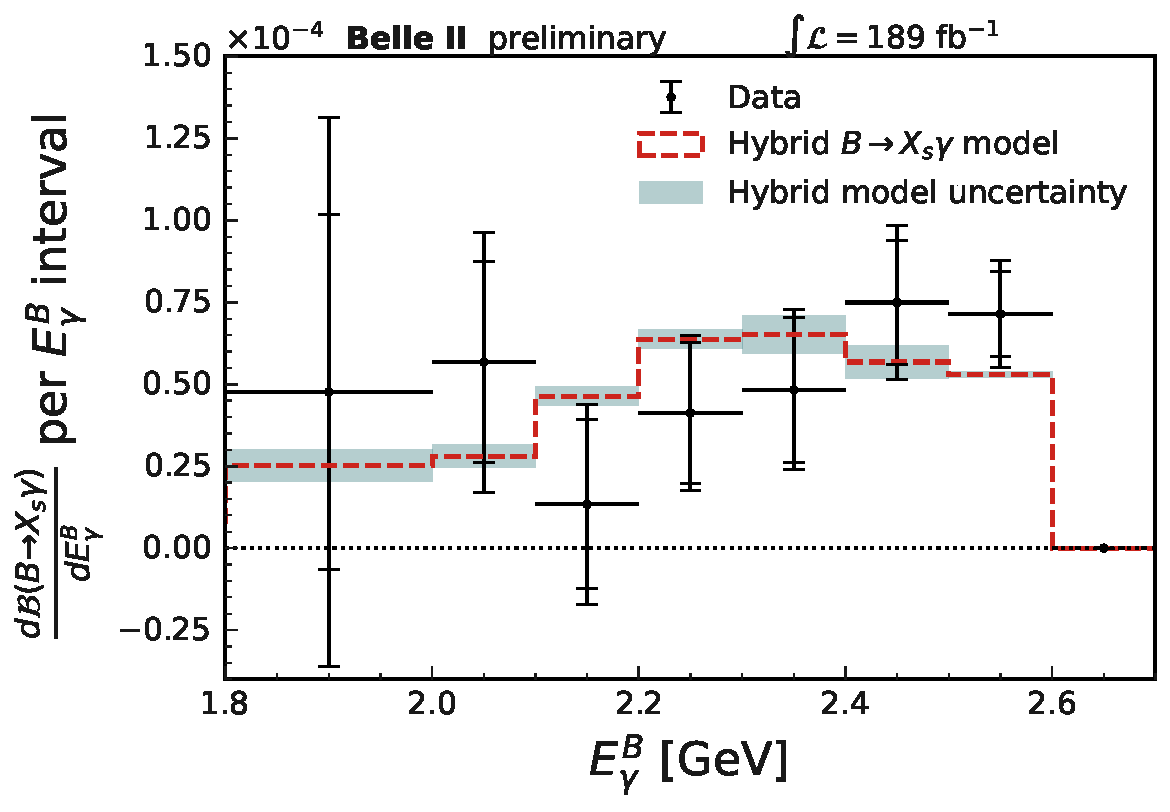
\includegraphics[width=0.45\textwidth]{figures/final_results/partial_bfs.pdf}
    }
    \subcaptionbox{\label{fig:correlation_uncertainty_matrix}}{
        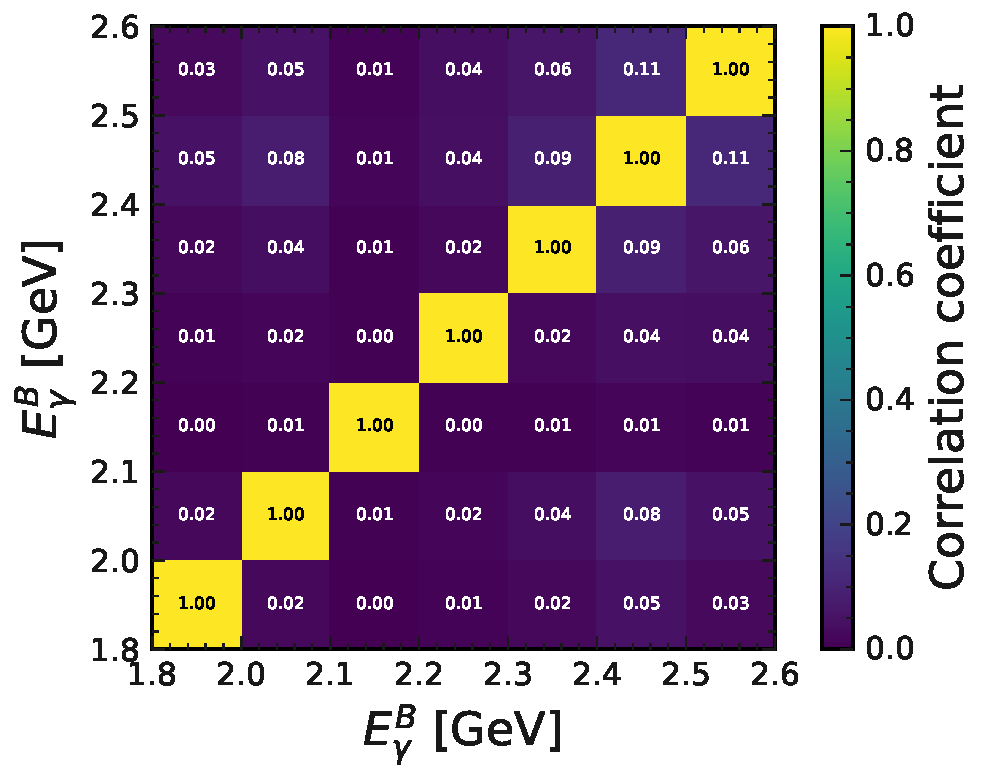
\includegraphics[width=0.45\textwidth]{figures/final_results/correlation_matrix_uncertainties.pdf}
    }
    \caption{\label{fig:partial_and_correlation} 
    The visualisation of results in  \Cref{tab:partial_branching_fractions}.
    \Cref{fig:partial_branching_fraction} shows th epartial branching fractions of \BtoXsgamma 
    as a function of \EB, measured in 189~\invfb Belle~II data.
    The inner error bars correspond to the statistical uncertainty, whereas the outer ones to the total.
    The measurement results are overlaid with the expectations for the hybrid signal-model, and the associated uncertainty to it, evaluated in \Cref{sec:signal_model}.
    The data results show excellent agreement with the model.
    \Cref{fig:correlation_uncertainty_matrix} shows 
    the correlation matrix of the partial branching fraction uncertainties.
    The systematic and statistical correlation is combined.
    As the results are statistically dominated, the correlations between different \EB bins are low.
    }
\end{figure}

\subsection{Total branching fraction measurement results}\label{sec:total_branching_fraction_results}

As the measurement employs a selection of $\EB>1.4~\gev$, a full $\mathcal{B}(\BtoXsgamma)$ cannot be measured.
Furthermore, the $\EB\in(1.4,1.8)~\gev$ range has a low precision, with a large systematic and statistical uncertainty component.
Therefore, only an evaluation in the $\EB\in(1.8,2.6)~\gev$ interval from experimental data is feasible.
The results for thresholds of $1.8~\gev$, $2.0~\gev$ and $2.1~\gev$ are given in \Cref{tab:integrated_branching_fractions}.
Because of correlation of systematic uncertainties, they become dominant at the lowest-\EB threshold, but remain comparable to the statistical uncertainty.

To compare with the results of other experiments and theoretical values,
one can use the theoretical extrapolation factors provided in Ref. \cite{Buchmuller:2005zv},
to evaluate the branching fraction at the threshold of $\EB>1.6~\gev$.
As it was discussed in \Cref{sec:btosgamma_totalrate_theory}, for \BtoXsgamma total rate evaluation, $\EB>1.6~\gev$ is a conventionally chosen threshold.
The extrapolated results are also provided in the last column on \Cref{tab:integrated_branching_fractions}.

\begin{table}[htbp!]
    \centering
    \caption{\label{tab:integrated_branching_fractions}
    The integrated \BtoXsgamma branching fractions for different lower-\EB threshold measured on $189~\invfb$ of Belle~II data.
    They are evaluated by summing the partial branching fractions in \Cref{tab:partial_branching_fractions}.
    The systematic and statistical uncertainties are denoted in the brackets.
    }
    \resizebox{1\textwidth}{!}{
    \begin{tabular}{ccl}
    \hline
        \EB lower threshold [\hspace{-1pt}$\gev$] & 
        $\mathcal{B}(B\rightarrow X_s \gamma)~[10^{-4}]$ & 
        \makecell{$\mathcal{B}(B\rightarrow X_s \gamma)~[10^{-4}]$\\(extrapolated to $1.6~\gev)$ \cite{Buchmuller:2005zv}} \\
        \hline
            $1.8$  & $3.54 \pm 0.78$ (stat.) $\pm~0.83$ (syst.) & $3.65 \pm 0.80$ (stat.) $\pm 0.86$ (syst.) $\pm 0.02$ (extrap.)\\ 
            $2.0$  & $3.06 \pm 0.56$ (stat.) $\pm~0.47$ (syst.) & $3.42 \pm 0.62$ (stat.) $\pm 0.52$ (syst.) $\pm 0.06$ (extrap.)\\
            $2.1$  & $2.49 \pm 0.46$ (stat.) $\pm~0.35$ (syst.) & $2.86 \pm 0.53$ (stat.) $\pm 0.40$ (syst.) $\pm 0.08$ (extrap.)
            \textsuperscript{1} \\
        \hline
    \end{tabular}

}
\end{table}

The results presented in \Cref{sec:results} are the main goal of the analysis.
The discussion related to them, their interpretation and future prospects for \BtoXsgamma will be discussed in \Cref{ch:overview}.

\footnotetext[1]{The extrapolation factor is not provided for $\EB=2.1~\gev$ threshold in \cite{Buchmuller:2005zv}.
                This result is evaluated by extrapolating linearly and assuming a monotonic increase in uncertainty.
                This results in an extrapolation factor $0.870\pm0.024$. 
                The number should be interpreted with the aforementioned caveats in mind only.}


\subsection{Moments of the \safeBtoXsgamma photon-energy spectrum}\label{sec:spectrum_moments}

As discussed in \Cref{sec:btosgamma_totalrate_theory,sec:btosgamma_spectrum_theory} the moments of the \BtoXsgamma
spectrum are important for the understanding of \BtoXsgamma decay properties.
The first and second moment of the \BtoXsgamma spectrum are calculated based on the results in \Cref{tab:partial_branching_fractions}.
They are approximated as a weighted sum of the center value of \EB intervals, $\mathrm{\Delta\EB}$,
with weights corresponding to the partial branching fractions in that \EB interval:
\begin{align}\label{eq:weighted_sum_moments}
    \begin{split}
        \expval{\EB} &= \frac{\sum_i f_c(\Delta\EB^{}_{,i})\times  
                               \frac{\Delta\mathcal{B}(\BtoXsgamma)_i}
                                    {\Delta {E^B_{\g}}_{,i}}}
                             {\sum_i \frac{\Delta\mathcal{B}(\BtoXsgamma)_i}{\Delta {E^B_{\g}}_{,i}}},
    \end{split}
\end{align} 
where $f_c$ is used as a loose notation for a function that returns the center point of an interval.
The calculated values of the first and second moments of \EB for different lower thresholds are given in \Cref{tab:moments}.
The systematic and statistical uncertainties are match those in earlier subsections, and their correlation is accounted as discussed before.

Note that the results strongly depend on the threshold -- particularly for the second moment.
The measured values of the first moment in \Cref{tab:moments} (average of the photon energy spectrum) slightly decrease with the \EB threshold as additional
low energy \EB intervals bring the value lower.
The total uncertainty changes from 2\% to 4\% as the \EB lower threshold decreases from 2.1~\gev to 1.8~\gev.
On the other hand, the second moment (the variance of the spectrum) highly depends on the threshold chosen, 
and the uncertainties grow swiftly with a decreasing \EB threshold.
While the uncertainty with a 2.0~\gev \EB threshold is at 25\%, this increases to 46\% at 1.8~\gev.
A larger uncertainty is attributed to the fact that the dispersion of the possible \EB energies highly depends on a precise measurement of the tail,
whereas in the case of the first-moment the peak region carries the highest importance.


\begin{table}[htbp!]
    \centering
    \caption{\label{tab:moments}
    The integrated \BtoXsgamma first and second moments for different lower-\EB threshold measured on $189~\invfb$ of Belle~II data.
    They are evaluated by a weighted sum of the the partial branching fractions in \Cref{tab:partial_branching_fractions} according to \Cref{eq:weighted_sum_moments}.
    The systematic and statistical uncertainties are denoted in the brackets.
    }
    \resizebox{1\textwidth}{!}{
    \begin{tabular}{|c|cc|}
    \hline
        \EB lower threshold [\hspace{-1pt}$\gev$] & 
        $\expval**{\EB}$ [$\gev$] & $\expval**{\EB^2}$ - $\expval**{\EB}^2$ [$\gev^2$]\\
        \hline
        1.8 & 2.284 $\pm$ 0.065 (stat.) $\pm$ 0.071 (syst.)    & 0.0502 $\pm$ 0.0157 (stat.) $\pm$ 0.0176 (syst.)\\
        2.0 & 2.343 $\pm$ 0.036 (stat.) $\pm$ 0.026 (syst.)    & 0.0315 $\pm$ 0.0063 (stat.) $\pm$ 0.0045 (syst.)\\
        2.1 & 2.410 $\pm$ 0.032 (stat.) $\pm$ 0.019 (syst.)    & 0.0147 $\pm$ 0.0057 (stat.) $\pm$ 0.0036 (syst.)\\
        
        \hline
    \end{tabular}

}
\end{table}
